\documentclass[preprint,12pt]{elsarticle}

%General Short-Cut Commands
\newcommand{\superscript}[1]{\ensuremath{^{\textrm{#1}}}}
\newcommand{\subscript}[1]{\ensuremath{_{\textrm{#1}}}}
\newcommand{\nuc}[2]{\superscript{#2}{#1}}
\newcommand{\ith}[0]{$i$\superscript{th}}
\newcommand{\jth}[0]{$j$\superscript{th}}
\newcommand{\kth}[0]{$k$\superscript{th}}

% New definition of square root:
% it renames \sqrt as \oldsqrt
\let\oldsqrt\sqrt
% it defines the new \sqrt in terms of the old one
\def\sqrt{\mathpalette\DHLhksqrt}
\def\DHLhksqrt#1#2{%
\setbox0=\hbox{$#1\oldsqrt{#2\,}$}\dimen0=\ht0
\advance\dimen0-0.2\ht0
\setbox2=\hbox{\vrule height\ht0 depth -\dimen0}%
{\box0\lower0.4pt\box2}}

\usepackage{natbib}
%\bibpunct[,]{[}{]}{;}{a}{,}{,}
\bibliographystyle{model2-names}

% Needed for making certian figures
\usepackage{color}
\usepackage{tikz}
\usepackage{verbatim}
\usetikzlibrary{shapes,arrows}

\journal{Some Separations Journal}

% Start this document...
\begin{document}

% Article commands
\begin{frontmatter}
\title{Symbolic Multicomponent Enrichment for Matched Abundance Ratio Cascades}

\author[chi]{Anthony M. Scopatz\corref{cor1}}
\ead{scopatz@flash.uchicago.edu}
\cortext[cor1]{Corresponding author}

\address[chi]{The University of Chicago, The FLASH Center, 
              5754 S. Ellis Ave, Chicago, IL, 60637}


% Text of abstract
\begin{abstract}
Some abstract text
\end{abstract}

%% keywords here, in the form: keyword \sep keyword
\begin{keyword}
%% MSC codes here, in the form: \MSC code \sep code
%% or \MSC[2008] code \sep code (2000 is the default)
\end{keyword}

\end{frontmatter}


%
% Begin real text
%

\section{Introduction}
\label{sec:intro}
Symbolic evaluation is slow, except...


\section{Symbolic Methodology}
\label{sec:meth}
At its core, the solution to coupled multicomponent enrichment cascade equations is
a minimization problem \cite{Wood1999}.  In a matched abundance ratio 
\cite{DelaGarza1969} cascade this is often cast as the minimization of 
the total flow rate $L$ through the system normalized by the feed flow rate $F$ to 
form the positive and unitless optimization variable $L/F$.  Traditionally, 
minimizing this parameter as a function of other cascade state variables has been 
performed eiether via off-the-shelf optimization libraries 
\cite{doi:10.1080/01496391003793884} or custom built solvers CITEpyne.

However, both of these approaches rely on writing code idiomatic to underlying 
programming language.  For example, many numerical constraint optimizers, in order 
to handle the case of arbiratily complex expressions, accept as their primary 
argument a function object or pointer.  Then for every iteration the optimizer must 
call the function to be optimized.  This involves (in compiled languages) setting up 
a new stack and allocating new memory for every solver iteration.  While good 
optimizers will be effieicnt in terms of the number of function calls they make, 
there is no way for them to avoid multiple function calls and remain sufficiently 
general. The number of function calls that are needed scales \emph{at least} linearly 
with the number of equations in the system.

On the other hand, if it is possible to convert the system of equations 
into a single expression -- no matter how complicated -- then the problem has been 
recast into the optimization of a single fucntion over a single variable.   This 
may be easily handed off to any number of well known algorithims, such as Newton's
method, the secant method, or the bisection method.  In such a form, the solution 
will have a vastly reduced computational overhead as compared to standard 
numerical solvers. 

Naturally, performing the above variable substitution and elimination to obtain a 
single expression is difficult in many cases and mathematically impossible in most 
others.  For MARC systems, as is shown in \S \ref{sec:symes}, reduction of $L/F$
to a single expression is possible.

Rather than phrasing this as a numerical optimization problem from the start, the 
opposite conceptual tactic is taken.  The MARC system is expandend, manipulated, 
and subsititued symbolically the the majority of the calculation.  The actual 
numerical results of the calculation are only computed as needed as the final step.
The symbolic manipulation is generated prior to compilation, resulting in 
very fast run time solutions.

In \S \ref{sec:marceq} the standard MARC system of equations is detailed. 
Then the novel reinterpretation of the MARC equations is related in 
\S \ref{sec:symes}.  
Lastly, \S \ref{sec:codegen} characterizes the pipeline that takes the symbolic MARC 
eqautions and converts them into fast machine code.  
For the remainder of \S \ref{sec:meth}, a three-component natural uranium fed 
cascade will be used when example data is required.
Higher order cascades will be discussed in \S \ref{sec:res}.

\subsection{MARC Equations}
\label{sec:marceq}
The algorithm with which to compute matched abunance ratio cascades has been 
detailed previously in a vareity sources, dating back to de la Garza in the
1960s. However, the fundementals of this method are reviewed here both as a formal
statement of the problem and as a way to introduce the terminology used throughout 
the rest of this paper.  For more information please refer to de la Garza
\cite{DelaGarza1969}, von Halle \cite{VonHalle1987}, Wood \cite{Wood1999}, or 
Song \cite{doi:10.1080/01496391003793884}.

Call $N$ the total number of stages in an enrichment cascade, $N_P$ the number of 
product (enriching) stages above the feed entry, and $N_T$ the number of tails
(stripping) stages below the feed point such that:
\begin{equation}
N = N_P + N_T
\end{equation}
Furthermore, MARC requires that we declare a species to enrich in the 
product (subscript P).  This is known as the first key component an is denoted 
here as $j$.  There must also be a second key component $k$ from which $j$ is 
separated. Thus $k$ is more abundant in the tails stream (subscript T).

The ovearll stage separation factor $\alpha$ [unitless] represents the per mass 
enrichment ratio from one stage to the next.  This yeilds component-specific
stage separation factors $\beta_i$ for the \ith component of a mixture $I$:
\begin{equation}
\beta_i = \alpha^{M^* - M_i}
\label{beta_i}
\end{equation}
Here, $M_i$ represents the molecular weight [amu] of the \ith
species while $M^*$ [amu] is an optimization parameter.  An initial first guess for 
$M^*$ is given by the average of the molecular weights of the key components:
\begin{equation}
M^* = \frac{1}{2}\left(M_j + M_k\right)
\label{mstar-guess}
\end{equation}
By convention, $j$ \& $k$ are chosen such that $M_j < M_k$ and 
therefore $M^*$ is bounded on the range $M^*\in[M_j,M_k]$ when minimizing $L/F$.

Let $F$, $P$, and $T$ be the feed, product, and tails mass flow rates subject to 
the conservation equation:
\begin{equation}
F = P + T
\label{total-flow-constraint}
\end{equation}
Also let $x$ denote a normalized mass concentration vector such that $x_i^F$, 
$x_i^P$, $x_i^T$ are the concetrations of the \ith component of the feed, product,
and tails respectively.  Thus:
\begin{equation}
1 = \sum_i^I x_i^F = \sum_i^I x_i^P = \sum_i^I x_i^T 
\end{equation}
Therefore the flow rate ratios are:
\begin{equation}
\frac{P}{F} = \sum_i^I x_i^F\frac{\beta_i^{N_T+1} - 1}
                                 {\beta_i^{N_T+1} - \beta_i^{-N_P}}
\label{ppf-full}
\end{equation}
\begin{equation}
\frac{T}{F} = \sum_i^I x_i^F\frac{1 - \beta_i^{-N_P}}
                                 {\beta_i^{N_T+1} - \beta_i^{-N_P}}
\label{tpf-full}
\end{equation}
Equations \ref{ppf-full} \&  \ref{tpf-full} can be further reduced to functions
of just the first key component:
\begin{equation}
\frac{P}{F} = \frac{x_j^F - x_j^T}{x_j^P - x_j^T}
\label{ppf-key}
\end{equation}
\begin{equation}
\frac{T}{F} = \frac{x_j^F - x_j^P}{x_j^T - x_j^P}
\label{tpf-key}
\end{equation}

Either equations \ref{ppf-full} \& \ref{tpf-full} or equations \ref{ppf-key} \& 
\ref{tpf-key} allow the calculation of the \ith component concentrations of in the 
product and tails streams as a function of the feed concentrations.
\begin{equation}
x_i^P = \frac{x_i^F}{\frac{P}{F}}\cdot\frac{\beta_i^{N_T+1} - 1}
                                           {\beta_i^{N_T+1} - \beta_i^{-N_P}}
\label{prod-concentration}
\end{equation}
\begin{equation}
x_i^T = \frac{x_i^F}{\frac{T}{F}}\cdot\frac{1 - \beta_i^{-N_P}}
                                           {\beta_i^{N_T+1} - \beta_i^{-N_P}}
\label{tail-concentration}
\end{equation}
By analogy to equation \ref{total-flow-constraint}, the components themselves are
also subject to mass conservation:
\begin{equation}
x_i^FF = x_i^PP + x_i^TT
\label{comp-flow-constraint}
\end{equation}

What gives MARCs their moniker, however, is that at every stage any two flows of 
the same type ($F$, $P$, \& $T$) must produce the same relative concentrations of 
the two key components.  Call $R$ an abundance ratio.  Then for matched abundance 
ratio cascades, 
\begin{equation}
R^F = \frac{x_j^F}{x_k^F}; \;\;\; R^P = \frac{x_j^P}{x_k^P}; \;\;\; 
R^T = \frac{x_j^T}{x_k^T}
\label{abund_ratios}
\end{equation}
The ratios in equation \ref{abund_ratios} are valid for the three stages in the 
cascade that are most important: the feed entry point, the final product, and the 
last tails stage.

Finally, the total flow rate per unit feed for a given cascade is computed by 
the following expression:
\begin{equation}
\frac{L}{F} = \sum_i^I \frac{\frac{P}{F}x_i^P\ln(R^P) + \frac{T}{F}x_i^T\ln(R^T) 
                                                      - x_i^F\ln(R^F)}
                            {\ln(\beta_j)\frac{\beta_i - 1.0}{\beta_i + 1.0}}
\label{ltot-over-feed}
\end{equation}
To solve for the optimal cascade, equation \ref{ltot-over-feed} must be minimized
with respect to its constituent independent variables.

Suppose that the cascade parameters 
$\alpha$, 
$j$, $k$, 
$M_i$ for all $i$, 
$x_i^F$ for all $i$, 
the key product enrichment $x_j^P$, and the key 
tails enrichment $x_j^T$ are all given.  The optimal cascade is thus characterized by 
the system of equations below. This system has three equations and three unknowns --
$N_P$, $N_T$, and $M^*$ -- and is therefore well determined.
\begin{equation}
\frac{x_j^P}{x_j^F}\cdot\frac{P}{F} - \frac{\beta_j^{N_T+1} - 1}
                                           {\beta_j^{N_T+1} - \beta_j^{-N_P}} = 0
\label{prod-constraint}
\end{equation}
\begin{equation}
\left(\frac{x_j^F}{\frac{T}{F}} \cdot \frac{1 - \beta_i^{-N_P}}
                                           {\beta_j^{N_T+1} - \beta_j^{-N_P}} \right)
- \left(x_j^T\cdot\sum_i^{I} x_i^T\right) = 0
\label{tail-constraint}
\end{equation}
\begin{equation}
\min\left[\frac{L}{F}\right]\to \frac{d}{dM^*} \frac{L}{F} = 0
\label{minlt-constraint}
\end{equation}
Equation \ref{prod-constraint} is a rearrangement of equation \ref{prod-concentration}
when evaluated for the \jth key component, whose product erichment is assumed
known.  Equation \ref{tail-constraint} is garnered via equations \ref{tpf-full} \&
\ref{tail-concentration} and once again evaluated for the \jth key component.
Equation \ref{minlt-constraint} falls out of the extreme value theorem of calculus
applied to equation \ref{ltot-over-feed}.

To solve equations \ref{prod-constraint}-\ref{minlt-constraint}, initial guesses
for the number of product and tails stages, $N_P^0$ and $N_T^0$, must be given.
An initial guess for $M*$ is provided in equation \ref{mstar-guess}.  Once this system
of equations is known, the product and tails concentrations for all components may be 
solved with equations \ref{prod-concentration} \& \ref{tail-concentration}.

\subsection{Symbolic Enrichment Solver}
\label{sec:symes}

When solving a system of equations, it is advantageous if any of the independent 
variables has a closed form representation in terms of the other independent 
parameters. This is because the closed form reprsentation may be subtituted into 
the remaining equations and this variable eliminated from the computation.  This
transorms the system from $X$ equations with $X$ unknowns into a system with 
$(X-1)$ equations and $(X-1)$  unknowns.  Ideally, the system would then be reducible 
to one equation (with potentiall many substitutions) as a function of one unknown.

The symbolic MARC algorithm here relies on eliminating the $N_P$ and $N_T$ variables
from equations \ref{prod-constraint}-\ref{minlt-constraint}. This produces a single
expression for $L/F$, which may be handed to a traditional minimization algorithm.
Still, the strategy for devising a successful symbolic solver for a given system
of equations is distinct from the normal mechnisms used when engineering numeric 
solutions.

Unlike numeric solvers where every expression is evaluated with an integer, real, or
complex number as it is encountered, symbolic computation represents and stores all 
opperations performed on an expression.  Only after the accumulation of all 
opperations, and only if desired by the user, is a symbolic expression ever numerically
evaluted.  This is true even for compound operators such as triginometric functions, 
differentiaition, and integration.

Therefore certain operators (e.g. differentiation) may explode the number of binary
opperations in the resultant expression after their application (e.g. the chain rule).
So while the quintessential strategy in numerical evaluators is to mitigate error
steming from floating point arithmetic, a symbolic solver seeks to minimize the total
number of irreducible operation ($+, -, \times, /, \%, \log, \sin, \mbox{abs},$ etc.) 
which must be perfomed to compute a complex expression.  Hence much of the variable
elimination below also attempts to simeltaneously curtail the overall operation count. 

To start, consider the constraint in equation \ref{prod-constraint}, the key 
component simplification of $P/F$ seen in equation \ref{ppf-key}, and the number
of tails stages $N_T$.  As call to SymPy's \texttt{solve()} function rearranges the 
constraint to reveal the closed form solution $N_T(N_P, M^*)$:
\begin{equation}
\begin{array}{lcl}
N_T & = & \left[- M^{*} N_{P} \log{\left (\alpha \right )} - M^{*} \log{\left (\alpha \right )} + M_{j} \log{\left (\alpha \right )} - \log{\left (x^{T}_{j} \right )} \right. \\ 
& & \left. - \log{\left (\frac{- x^{F}_{j} + x^{P}_{j}}{\alpha^{M^{*} N_{P}} x^{F}_{j} x^{P}_{j} - \alpha^{M^{*} N_{P}}x^{F}_{j} x^{T}_{j} - \alpha^{M_{j} N_{P}} x^{F}_{j} x^{P}_{j} + \alpha^{M_{j} N_{P}} x^{P}_{j} x^{T}_{j}} \right )} \right] \\
& & \times \left[\left(M^{*} - M_{j}\right) \log{\left (\alpha \right )} \right]^{-1}
\end{array}
\label{nt_closed_full}
\end{equation}
While equation \ref{nt_closed_full} is successfully only a function of known 
parameters and $N_P$ and $M^*$, it is not an ideal expression.  This is because both 
$M^*$ and $N_P$ each appear five times in this closed form solution.  Thus if this 
were substitued into the original MARC system to eliminate $N_T$, the number of 
instances of indpendent variables would grow by a ratio of 10:1.    

To decrease the substitution ratio, and simplify the expression, equation 
\ref{nt_closed_full} may be rewritten (by hand) as the following:
\begin{equation}
\begin{array}{lcl}
N_T & = & \left[M^{*} \log{\left (\alpha \right )} - M_{j} \log{\left (\alpha \right )} + \log{\left (x^{T}_{j} \right )} + \log{\left (\frac{-1.0 + \frac{x^{P}_{j}}{x^{F}_{j}}}{x^{P}_{j} - x^{T}_{j}} \right )}  \right. \\
& & \left. - \log{\left (\frac{\alpha^{N_{P} \left(- M^{*} + M_{j}\right)} \left(x^{F}_{j} x^{P}_{j} - x^{P}_{j} x^{T}_{j}\right)}{- x^{F}_{j} x^{P}_{j} + x^{F}_{j} x^{T}_{j}} + 1 \right )}\right] \times \frac{1}{\left(- M^{*} + M_{j}\right) \log{\left (\alpha \right )}} \\
\end{array}
\label{nt_closed}
\end{equation}
Note that this transformation requires the logarithm identity 
$\log(a+c) = \log(a) + \log(1 + \frac{c}{a})$.  Equation \ref{nt_closed} is superior
in the sense that it requires 31 operations to as opposed to the original 38.
More importantly, $N_P$ appears only once in this 
expression and $M^*$ is reduced to three occurances.

\begin{figure}[htpb]
\begin{center}
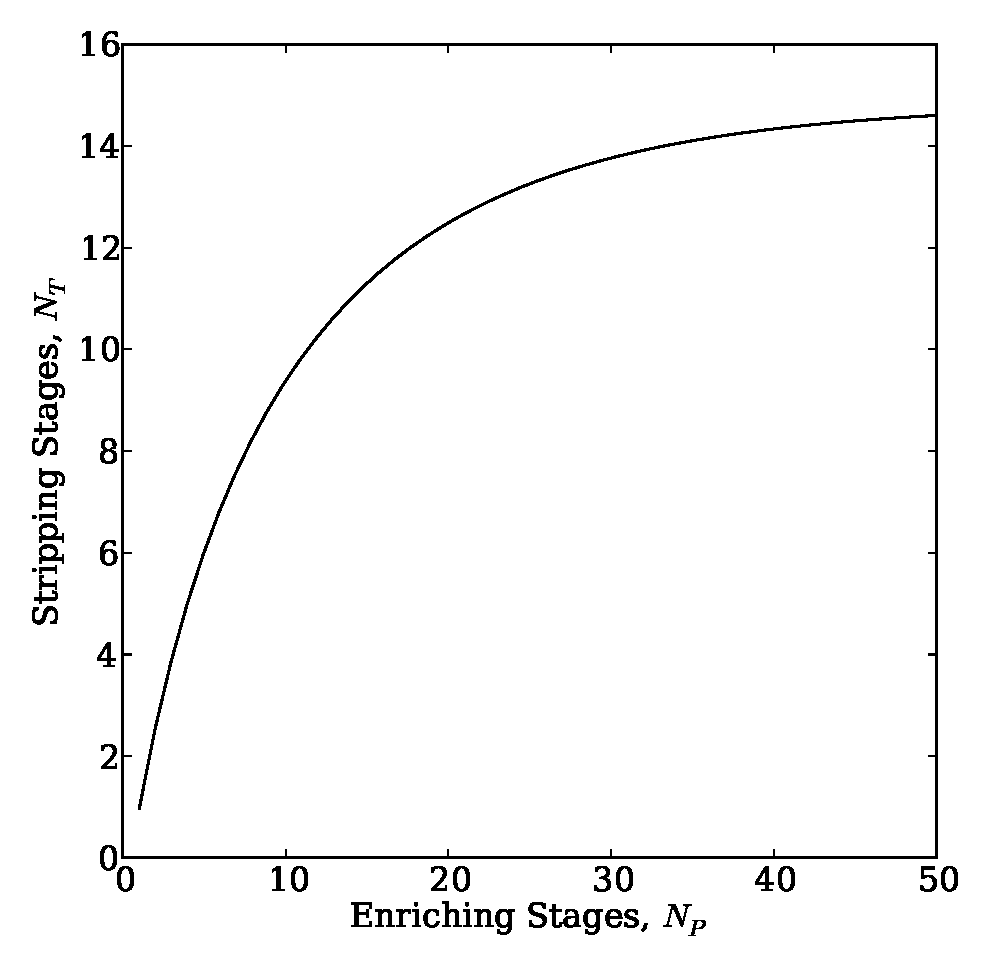
\includegraphics[scale=0.5]{nt_closed.eps}
\caption{$N_T(N_P, M^*)$ for a Natural Uranium Cascade with $N_P\in[1,50]$ and $M^*=236.547$.}
\label{nt_closed_fig}
\end{center}
\end{figure}

Figure \ref{nt_closed_fig} confirms that the closed form $N_T(N_P, M^*)$ is correct.
For an increasing number of enrichming stages, the stripping stages must also 
increase to maintain the proper matched abundance flow rates.
Therefore, equation \ref{nt_closed} allows for the elimination of $N_T$ as an 
independent variable when computing $L/F$ and $N_P$.

Next, examine the MARC constraint in equation \ref{tail-constraint}.  This states that
the tails concentraion of the \jth key component that is computed by the concentration
equations \emph{must} be equal to the concentraion specified for the cascade in the
initial conditions.  (Recall that $x_j^T$ is one of the known parameters.)  
Substituting $N_T(N_P, M^*)$ into this expression, the function $f$ is obtained:
\begin{equation}
f(N_P,M^*) =
\left(\frac{x_j^F}{\frac{T}{F}} \cdot \frac{1 - \beta_i^{-N_P}}
                                           {\beta_j^{N_T(N_P,M^*)+1} - \beta_j^{-N_P}} \right)
- \left(x_j^T\cdot\sum_i^{I} x_i^T\right) \equiv 0
\end{equation}
Here, like above with $P/F$, the key component simplification of $T/F$ in equation
\ref{tpf-key} is used.

Ideally, the terms in $f(N_P,M^*)$ would be rearrangable into a closed form expresssion
for either $N_P$ or $M^*$.  Since there are fewer instances of $N_P$, the number of
enriching stages would be the prefered candidate.  However from Galois theory, 
due to structure of $f(N_P,M^*)$ no such closed form solution is possible.  Examining
with respect to just $N_P$, the stucture of $f$ roughly fits:
\begin{equation}
\frac{1 + \alpha^{-N_P}}{\alpha^{-\log(\alpha^{-N_P})+1} - \alpha^{-N_P}} - x_j^T
    \frac{1 + \alpha^{-N_P}}{\alpha^{-\log(\alpha^{-N_P})+1} - \alpha^{-N_P}} -
    \cdots 
\end{equation}
Even this overly simplified representation cannot be rearranged as is to give a 
closed form function for $N_P$.  It may be possible to achive such an expression 
by making logarithm aproximations, such as $\log(a) \approx a - 1$ for $a\approx1$.  
This could 
eliminate some of the multiply nested powers of $N_P$ which would potentially yield
a closed form representation.  However, since the $\log$ terms appear in the exponent
of $\alpha$, any eror induded by these approximations would be compounded 
uncessarily.  Therefore this line of inquiry was not pursued further.

\begin{figure}[htpb]
\begin{center}
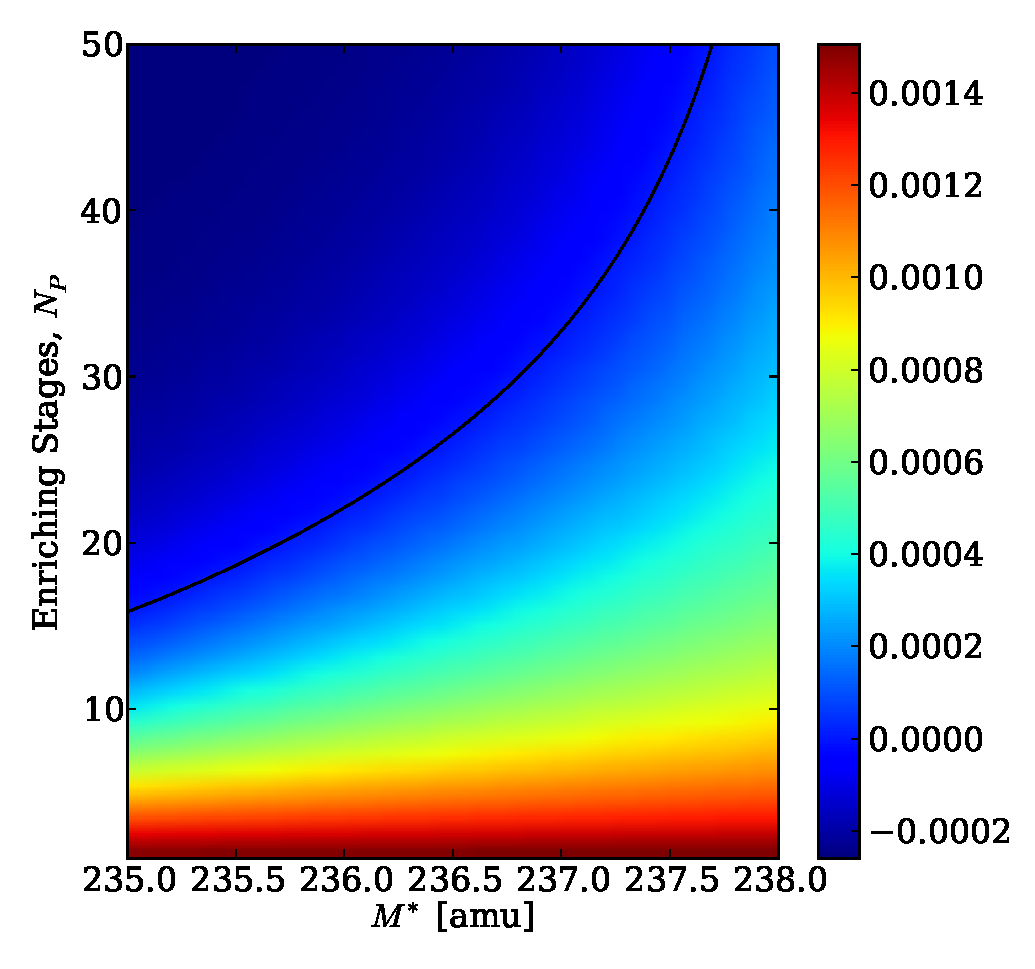
\includegraphics[scale=0.5]{np_constraint.eps}
\caption{$f(N_P, M^*)$ over the range of possible $N_P$ and $M^*$ values.  The black
countour line represents $f(N_P, M^*)=0$ and is the solution to the MARC contraint
in equation \ref{tail-constraint}. 
Data was computed for a typical natural uranium cascade.}
\label{np_contraint_fig}
\end{center}
\end{figure}

Instead, $f(N_P,M^*)$ was plotted as an unconstrained function of its two remaining 
indpendent variables to produce the heat map that may be seen in Figure 
\ref{np_contraint_fig}.  Since the range of $f$ contains both positive and negative
values, it follows that there must be some combination of $(N_P,M^*)$ values which
satisfy the original MARC constraint.  This set is displayed on Figure 
\ref{np_contraint_fig} as the black contour.  While this countour could hypothetically
be used itself to provide a closed form $N_P(M^*)$ equation, such a strategy would 
be grossly inefficient.  This is because a large number of $f$ points must be 
numerically evaluated, and then linerally interpoltated, to fit such a curve with
respectable accuracy.

Rather, by inspection of Figure \ref{np_contraint_fig}, the $f(N_P, M^*)=0$ curve 
would be well fit by a second order polynomial -- at least on the domain of interest.
That the constraint follows this form is not obvious from either equation 
\ref{tail-constraint} or $f(N_P,M^*)$.  Once again, however, the coefficients in 
such a second order polynomial model cannot be known numerically and must be 
expressed symbolically in terms of known and independent variables 
\cite{Sacks:1989:ASS:1623755.1623823}.

On these grounds, represent $f$ by its second order Taylor series expansion with
respect to $N_P$ close to the inital guess $N_P^0$.
\begin{equation}
\begin{array}{rcl}
f(N_P,M^*) & \approx &f(N_P^0,M^*) \\
& & + \left(N_P -N_P^0\right)\left.\frac{df}{dN_P}\right|_{N_P=N_P^0} \\
& & + \frac{\left(N_P -N_P^0\right)^2}{2}\cdot\left.\frac{d^2f}{(dN_P)^2}\right|_{N_P=N_P^0}\\
\end{array}
\label{f-taylor}
\end{equation}
This may be refactored with the introduction of coefficients $a$, $b$, and $c$ into 
the canonical form,
\begin{equation}
\begin{array}{rcl}
f(N_P,M^*) & = & a(N_P)^2 + bN_P + c\\
a & = & \frac{1}{2}\cdot\frac{d^2f}{(dN_P)^2}\\
b & = & \left.\frac{df}{dN_P}\right|_{N_P=N_P^0} - N_P^0\frac{d^2f}{(dN_P)^2} \\
c & = & f(N_P^0,M^*) - N_P^0\cdot\frac{df}{dN_P} + \frac{(N_P^0)^2}{2}\frac{d^2f}{(dN_P)^2} \\
\end{array}
\label{f-cannon}
\end{equation}
where all derivatives in equation \ref{f-cannon} are evaluated at $N_P=N_P^0$.
Applying the constraint $f(N_P,M^*)=0$, 
a closed form expression $N_P(M^*)$ is trivially solved for via the 
quadradic equation.
\begin{equation}
N_P(M^*) = \frac{-b - \sqrt{b^2 - 4ac}}{2a}
\label{np_closed}
\end{equation}
Note that for this approximation $a$ is always positive, $b$ is always negative, 
and the discrminant inside the sqaure root is always posiitve.  Therefore only the 
negative solution to the quadratic is needed to obtain a well-bounded result for
$N_P(M^*)$.

\begin{figure}[htpb]
\begin{center}
\begin{tabular}{cc}
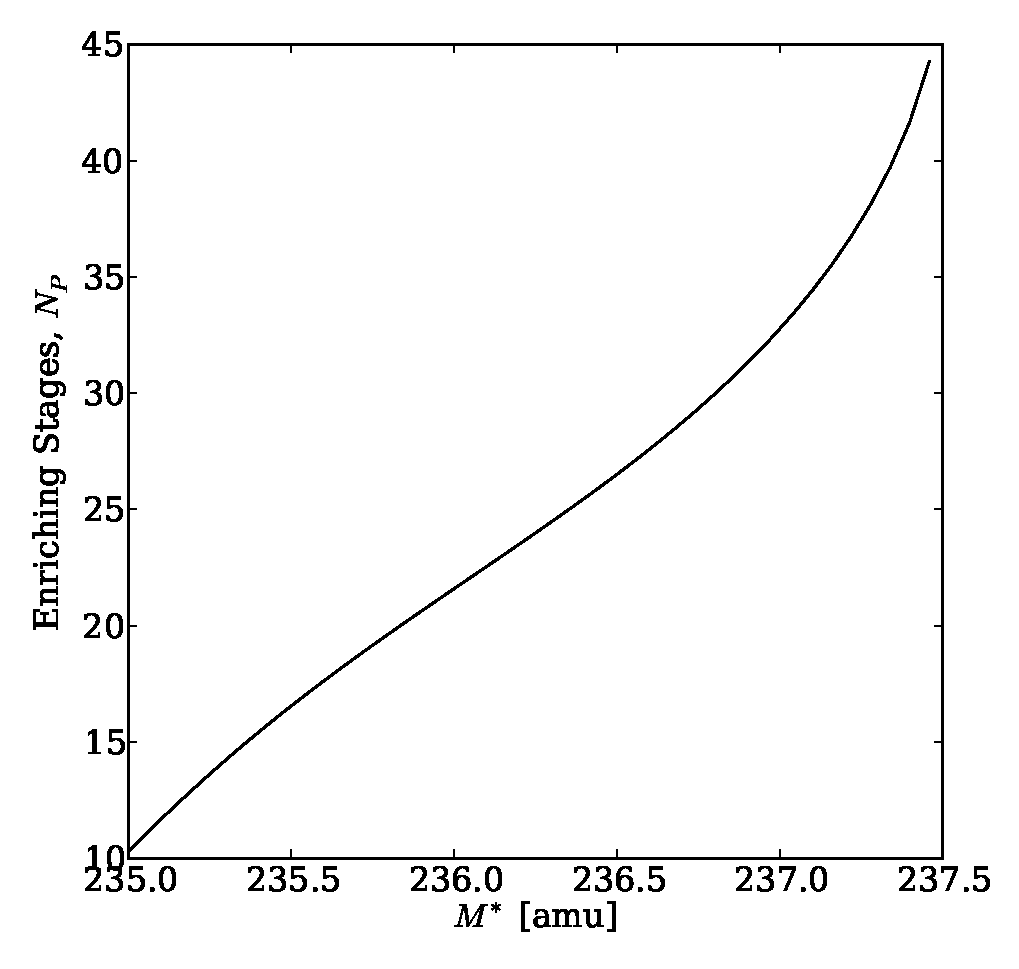
\includegraphics[scale=0.375]{np_closed.eps} & 
                                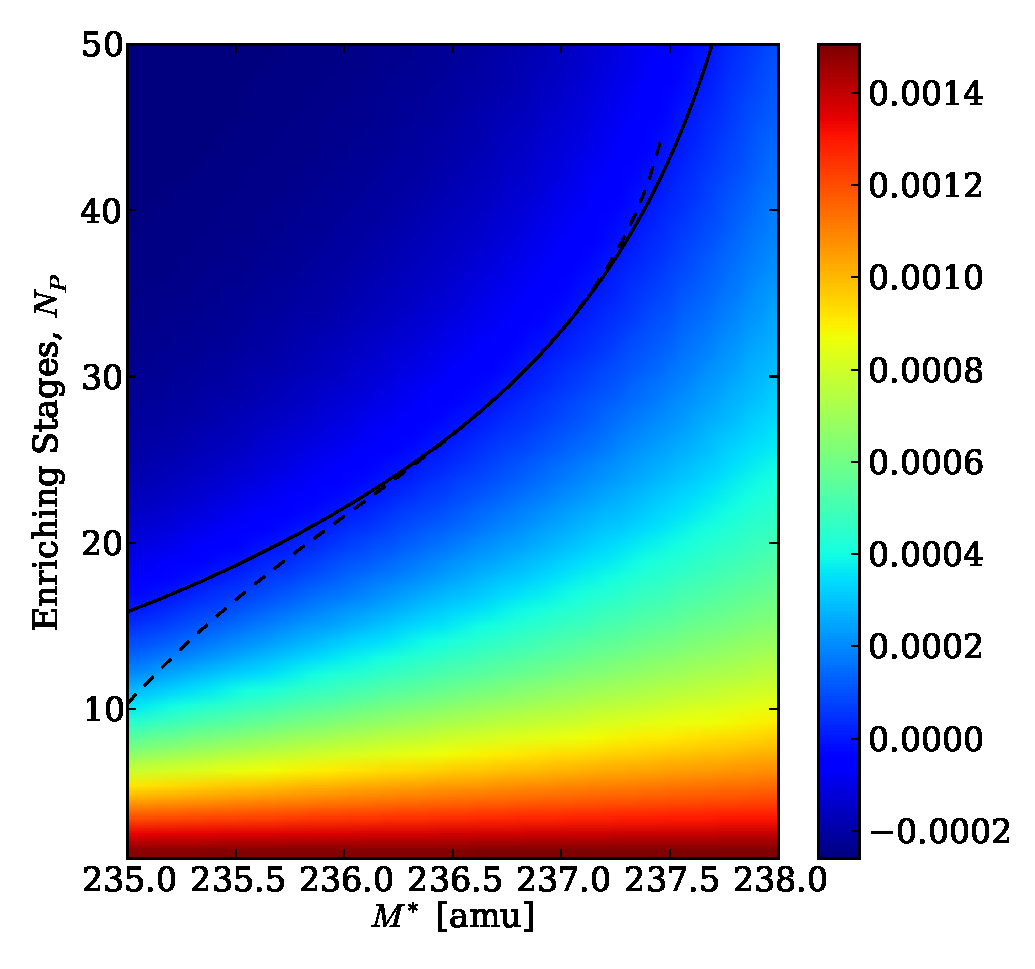
\includegraphics[scale=0.375]{np_closed_overlay.eps} \\
(a) & (b) \\
\end{tabular}
\caption{$N_T(M^*)$ such that $f(N_P,M^*)=0$.  (a): The quadradic solution to a
Taylor series approximation. Truncated when negative discriminants would result in
a complex solution.  (b): The equation from (a) as a dashed black line overlayed on top
of Figure \ref{np_contraint_fig}.  The solid black line is a linearlly interpolated
countour for $f(N_P, M^*)=0$. (a) \& (b) show that $N_P(M^*)$ is an accurate 
approximation near the intial guesses $N_P^0$ and $M^*=(M_j+M_k)/2$, but less 
precise far from this point. Data was computed for a typical natural uranium cascade.}
\label{np_closed_fig}
\end{center}
\end{figure}

Figure \ref{np_closed_fig} plots the closed form solution to $N_P(M^*)$ both (a)
on its own and (b) overlayed onto the above heat map.  This shows that the 
quadradic solution to the second order Taylor series approximation is an astondingly 
accurate one when close to the initial conditions $N_P=N_P^0$ and $M^*=(M_j+M_k)/2$.
Naturally being only second order, this approximation breaks down farther away from 
the initial guess.  For greater values of $N_P$ and $M^*$, the curve begins to 
over-predict the result until the point that the discriminat becomes negative, the
solution becomes complex, and the data set is truncated.  For smaller values, the
result diverges by under-predicting.  That $N_P(M^*)$ deviates at the edges of the
domain is an expected phenomenon for Taylor series approximations.

\begin{figure}[htpb]
\begin{center}
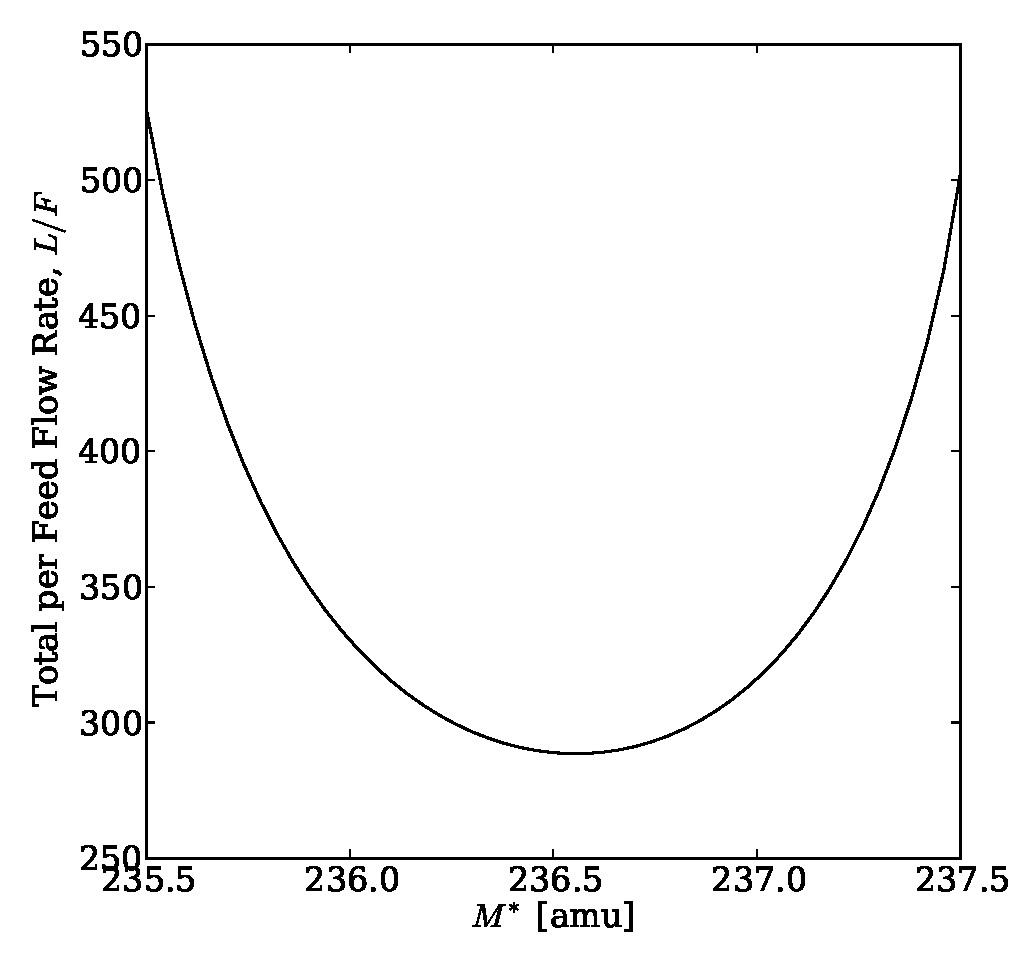
\includegraphics[scale=0.5]{loverf.eps}
\caption{$L/F(M^*)$ over the range of valid $M^*$ values.
Data was computed for a typical natural uranium cascade.}
\label{loverf_fig}
\end{center}
\end{figure}

Therefore, equation \ref{np_closed} may be substituted into equation \ref{nt_closed}
to obtain an expression $N_T(N_P(M^*),M^*)=N_T(M^*)$ which only depends on $M^*$ and 
the initial conditions.  Moreover, both equations \ref{nt_closed} \& \ref{np_closed}
may be subsititued into equation \ref{ltot-over-feed} to obtain 
$L/F(N_P(M^*),N_T(M^*),M^*)=L/F(M^*)$ solely as a function of $M^*$.  Thus
$L/F(M^*)$ may be minimized using any standard one-dimensional algorithm.
Figure \ref{loverf_fig} shows $L/F(M^*)$ for the full domain of $M*$, demonstrating 
that this symbolic methodology computes the correct bowl-like shape.  Note that while 
this method is successful, the number of operations in the final form of $L/T$ may be 
in the thousands to millions depending on how many components are included in the 
calculation.  A mechanism for mitigating huge numbers of opperations is described
in \S \ref{sec:codegen}.


\subsection{Code Generation Pipeline}
\label{sec:codegen}

Up until this point, all symbolic computations and manipulations have taken place
within SymPy.  For large numbers of operations -- such as the final expression for
$L/F(M^*)$ in \S\ref{sec:symes} -- SymPy becomes memory bound.  Therefore any 
minimization performed with SymPy would have unnessicaraly large overhead and would
not be computationally efficient.  For most symbolic solvers, this is where
methodolgy development ends.  Either the computation is small enough to not hit
memory limits and the calculation may proceed or it is too big and the evaluation
becomes untenable.  For the solver presented here, however, the computational 
pipeline is only in its initial step.

Symbolic mathematics libraries are ``slow'' and have a relatively large memory 
footprint because they must retain all operational information about an expression.
This is in preparation for possible further symbolic manipulation.  Numerical 
reduction and evaluation comes only when explicitly requested as it destroys the 
symbolic relationships.

Still, by the point that an expression for $L/F(M^*)$ has been determined, the 
desire to reatian the symbolic relationships is strongly outweighted by the hope
for fast execution times.  The system of equations has been solved and no further
symoblic manipulations will occur.

A tool which freezes in-place symbolic relationships and produces fast machine 
code is a compiler.  For purposes here any standard compiler (such as gcc, LLVM, or 
Intel) will sufice, though hardware specific compilers (such as OpenGL and CUDA)
also exist.  Most compiler collections support a number of intermeadiate languages
which may be used prior to machine code generation.  The \emph{de facto} contemporary
standard is C, or possibliy C++.

Having $L/F(M^*)$ and related equatrions for all other cascade parameters as 
symbolic expressions, the strategy implemented here takes this system and uses
it to generate C/C++ source code.  The C representation is then handed off to the
compiler of choice by the user.  The user may then access the compiled version
through a well-defined abstract programming interface (API) which accepts an initial
conditions cascade and returns the solved cascade.

Walking a symbolic expression tree to produce the coorespondeing C-code was performed 
with SymPy's own \texttt{codegen()} function.  However, this only assembles the 
code relevant to a single expression.  Therefore several calls to  \texttt{codegen()},
in the appropriate order, to generate a single C function representing the entire 
system of MARC equations.

It is important to note that the C-code which is generated is only an interim 
representation.  Therefore it need not be idiomatic, human-readable, or concise.
The only quality which matters is that it produce fast machine code upon compilation.
Thus some common features of modern compiled languages can and should be abset 
from the produced C-code.  These include an abscense of helper functions, an 
avoidance of accessing memory on the heap, the truancy of loop structures, and a
dearth of conditional branching.  In essence, the interim C representation should
hope to contain only variable assignment statements, jump statements, and 
arithmetic binary operations.

The above opperations are so blessed or condemded because of the number of clock
cycles on the processor they take.  For example, most arithmetic opertions take
1 - 5 processor instructions.  Jumps and assignment (on the stack) may each take
a single instruction.  Function calls, however, involve setting up a new stack
and may require 100+ cycles to execute.  Heap allocation, access, and deallocation
effectively amounts to function calls.  Conditional evaluation, which involves
processor branching, may take between 10 - 20 cycles.  Loop structures, while faster 
than fucntion calls, involve allocation of loop variables and possiblly conditional
checking.  Modern compilers may inline functions when indicated and attempt 
to unroll loops when possible, providing the associated speed boost.  However, 
since the C-code is already being generated, automatically inlining all potential
functions and unrolling all loops automatically ensures that produced machine code 
minimizes the number of clock cycles.  Trusting the compiler to cleverly optimize
source code must be done for hand written programs but is not required here.

Still, given the actual form of the equations it will not be possible to fully 
eliminate external function calls.  This is because the system includes logarithms, 
square roots, and powers which are implemented as functions in the C standard library.
Aside from these mathematical exceptions, though, additional function calls will
be avoided.

The above arguments being valid, it remains the case that fewer operations yields
shorter run times.  Thus it would be advantageous to reduce the total number of 
operations required prior to any compiled code generation.  Furthermore with the
similarity between many terms in the MARC equations, it stands to reasons that the
total number of operations could be drastically reduced.  An algorithm for 
caching and replacing common terms in an expression is known as common 
sub-expression elimination (CSE) \cite{Cocke:1970:GCS:390013.808480}.

As a simple CSE example, consider the following expression with $m$ and $n$ unknown:
\begin{equation}
\frac{m^{m+n+1} + n^{m+n+1} - 1}{m + n + 1} - m - n - 1
\label{cse-expanded}
\end{equation}
If instead $q$ is set such that,
\begin{equation}
\begin{array}{l}
q = m + n + 1\\
\frac{m^{q} + n^{q} - 1}{q} - q\\
\end{array}
\label{cse-condensed}
\end{equation}
then the total number of opperation in expression \ref{cse-expanded} is 14 as
opposed to the 9 operations in the system described by \ref{cse-condensed}.
General CSE algorthims are much more complex than this demonstration.  They are
therefore much more computationally expensive, typically at least $O(N^2)$, as
they must search over the space of all possible subsitituitions.  However pricey
CSE may be, it is still an upfront cost that is paid before C-code generation and
results in even faster machine-code.  Thus CSE is an essential step which cannot be 
avoided.  Here, SymPy's \texttt{cse()} function was used to reduce the overall 
number of operations.

\begin{figure}
\begin{center}
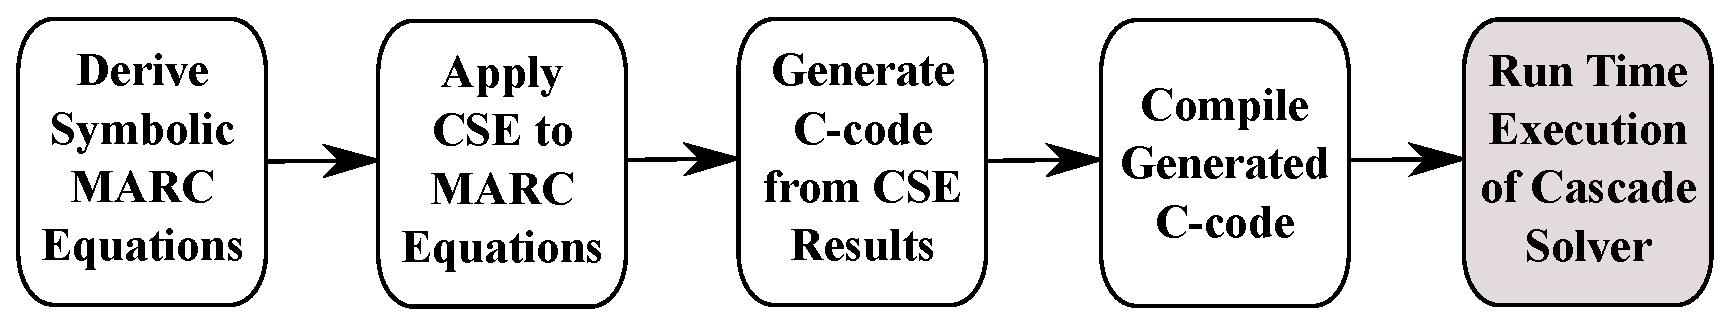
\includegraphics[scale=0.45]{codegen_pipeline.eps}
\caption{Flowsheet for fast machine code generation starting from initial symbolic MARC
equations.  Only the last step is executed at run time by the user.}
\end{center}
\label{codegen_pipeline}
\end{figure}

Bringing all of the above together, Figure \ref{codegen_pipeline} represents the 
code generation pipeline that takes the symbolic solution to the MARC equations
described in \S\ref{sec:symes} and converts them into optimized machine code.
This begins by taking the MARC equations and minimizes the number of opperations
by performing common sub-expression elimination.  Following this, non-idiomatic
C-code is produced.  This in turn is fed into a modern compiler.  Lastly, the compiled
code may be executed at run time with out needing to repreat any of the previous steps.

\section{Results \& Profiling}
\label{sec:res}
This section presents the results of the symbolic solution to the MARC system 
of equations after it has been transforms into fast executable code via the 
workflow described in \S\ref{sec:codegen}  Comparisons are made to both previously
published results as well and to idiomatic numerical solvers \& optimizers.  The 
comparison follows both the computation of the MARC cascade as well the $L/F$ 
minimization. Additionally, the code generation pipeline is profiled.  This gives a
heuristic indication of the large execution times that are avoided by generating 
code rather than remaining with a symbolic solution.

\subsection{MARC Solver}
\label{sec:l-solver}

To show that the symbolic method correctly solves for flow rates and concentrations,
consider the base case where no attempt is made to minimize $L/F$.  Rather, given 
an initial cascade setup the product and tails concentrations should be computed 
correctly.  A tungsten cascade example provided by E. von Halle is benchmarked against
here \cite{VonHalle1987}.

\begin{table}[htbp]
\begin{center}
\caption{Feed flow concentarations for a tungsten cascade via von Halle 
\cite{VonHalle1987}.}
\begin{tabular}{|l||c|}
\hline
\bf{Species} & \bf{von Halle $x^F$} \\ 
\hline
W180 & 0.00140 \\ 
\hline
W182 & 0.26416 \\ 
\hline
W183 & 0.14409 \\ 
\hline
W184 & 0.30618 \\ 
\hline
W186 & 0.28417 \\ 
\hline
\end{tabular}

\end{center}
\label{feed_vh}
\end{table}

Table \ref{feed_vh} displays the feed concentations for the sample tungsten cascade.
Additionally, this cascade has a static $M^*=181.0$, $N_P=35$, $N_T=14$,
$\alpha=1.16306$, \nuc{W}{180} as the \jth key component, \nuc{W}{182} as the \kth
key component, $x_j^P=0.51094$, and $x_j^T=0.00014$.  Tables \ref{prod_diff_vh} \&
\ref{tail_diff_vh} diplay the product and tails concentrations computed by von Halle, 
the symbolic solver, and the absolute differnece bewteen them.

\begin{table}[htbp]
\begin{center}
\caption{Product flow concentarations and differences for a tungsten cascade as 
computed by  von Halle \cite{VonHalle1987}, one pass through the symbolic solver, 
and two passes through the symbolic solver.  The second pass minimizes error arrising
from von Halle's cascade, which leaves $L/F$ unminimized.}
\begin{tabular}{|l||c||c|c||c|c|}
\hline
\bf{Species} & \bf{von Halle} & \bf{1 pass} & \bf{1 pass $\Delta$} & \bf{2 pass} & \bf{2 pass $\Delta$} \\ 
\hline
W180 & 0.51094 & 0.51172 & +7.7973e-04 & 0.51094 & -1.3003e-09 \\ 
\hline
W182 & 0.48756 & 0.48712 & -4.4296e-04 & 0.48789 & +3.3106e-04 \\ 
\hline
W183 & 0.00148 & 0.00115 & -3.2640e-04 & 0.00116 & -3.2077e-04 \\ 
\hline
W184 & 0.00002 & 0.00001 & -1.0368e-05 & 0.00001 & -1.0289e-05 \\ 
\hline
W186 & 0.00000 & 0.00000 & +1.3330e-10 & 0.00000 & +1.3528e-10 \\ 
\hline
\end{tabular}

\end{center}
\label{prod_diff_vh}
\end{table}

\begin{table}[htbp]
\begin{center}
\caption{Tails flow concentarations and differences for a tungsten cascade as 
computed by  von Halle \cite{VonHalle1987}, one pass through the symbolic solver, 
and two passes through the symbolic solver.  The second pass minimizes error arrising 
from von Halle's cascade, which leaves $L/F$ unminimized.}
\begin{tabular}{|l||c||c|c||c|c|}
\hline
\bf{Species} & \bf{von Halle} & \bf{1 pass} & \bf{1 pass $\Delta$} & \bf{2 pass} & \bf{2 pass $\Delta$} \\ 
\hline
W180 & 0.00014 & 0.00014 & -5.2751e-10 & 0.00014 & +8.8124e-16 \\ 
\hline
W182 & 0.26361 & 0.26361 & -4.9016e-07 & 0.26361 & -3.2463e-06 \\ 
\hline
W183 & 0.14444 & 0.14444 & +2.9159e-06 & 0.14444 & +3.4419e-06 \\ 
\hline
W184 & 0.30693 & 0.30694 & +5.9473e-06 & 0.30694 & +7.1036e-06 \\ 
\hline
W186 & 0.28488 & 0.28487 & -8.3725e-06 & 0.28487 & -7.2991e-06 \\ 
\hline
\end{tabular}

\end{center}
\label{tail_diff_vh}
\end{table}

Since the product enrichment of \nuc{W}{180} is almost 365 times larger than the feed
enrichment, it is reasonable to expect that the Taylor series approximation to 
$N_P(M^*)$ would be outside of its valid range.  (This, obviously, being an extreme
case.)  As is shown in Tables \ref{prod_diff_vh} \& \ref{tail_diff_vh}, however, 
even the worst case is off by no more than $7.8e-4$ in the product and $8.4e-6$ in the
tails.  

If tighter error bounds are desired, this is easily achivable by simply passing
the results for $N_P$ \& $N_T$ through the symbolic solver for a second pass, 
retatining all other cascade specifiations at their original values.  For all 
components which are not trivially small, the second pass reduces the magintude of the 
differences, in many cases dramatically so.  Note once again that such a second 
pass is only required for extreme enrichment jumps.  For more normal separations, 
this is not required.  Additionally such a pass is also not required when minimizing
$L/F$ since the top-level optimizer is already performing multiple passes.

Therefore even in the worst case scanrio described by von Halle, the symbolic 
solution to the MARC equations performs to within acceptable tolerance levels.


\subsection{$\min\left[L/F\right]$ Solver}
\label{sec:minl-solver}

The next step of the benchmark presented here is to verify that the minimization
of the total flow rate per unit feed has at least the same accuracy as 
numeric solvers.  Two cases are compared.  The first numeric solver was implemented 
using hand-written idiomatic C-code \cite{pyne:enrichment}.  The second case compares
minimum $L/F$ values with results publised by Song et al. 
\cite{doi:10.1080/01496391003793884}.

\begin{table}[htbp]
\begin{center}
\caption{Feed flow concentarations for a uranium re-enrichment cascade via  
    VISION \cite{Jacobson2009}.}
\begin{tabular}{|l||c|}
\hline
\bf{Species} & \bf{VISION $x^F$} \\ 
\hline
U234 & 0.00018 \\ 
\hline
U235 & 0.00819 \\ 
\hline
U236 & 0.00611 \\ 
\hline
U238 & 0.98552 \\ 
\hline
\end{tabular}

\end{center}
\label{feed_vision}
\end{table}

For the idiomatic C solver comparison, the same minimization algorthim was used.  
This is a modified implementation of Newton's method with automatically detects 
oscilations around the solution and, if necessary, decreases the tolerance.
The comparison was performed for a uranium cascade of material recovered from 
a light water reactor, which is then re-enriched.  The feed vector is taken from the
nuclear fuel cycle simulator VISION \cite{Jacobson2009}.

\begin{table}[htbp]
\begin{center}
\caption{Cascade parameter comparison after $L/F$ minimization for the symbolic 
    solver with a numeric solver (written in idiomatic C) using a uranium feed from 
    VISION \cite{Jacobson2009}.}
\begin{tabular}{|l||c|c|c|}
\hline
\bf{Parameter} & \bf{Symbolic} & \bf{Numeric} & \bf{Difference} \\
\hline
$L/F$ & 326.89566 & 326.89609 & -4.3245e-04 \\
\hline
$M^*$ & 236.58177 & 236.57897 & +2.8000e-03 \\
\hline
$N_P$ & 27.36549 & 27.33457 & +3.0923e-02 \\
\hline
$N_T$ & 15.02947 & 15.05036 & -2.0889e-02 \\
\hline
$x^P$ U234 & 0.00147 & 0.00147 & -2.2165e-07 \\
\hline
$x^P$ U235 & 0.05500 & 0.05500 & -2.9836e-06 \\
\hline
$x^P$ U236 & 0.02846 & 0.02845 & +4.8174e-06 \\
\hline
$x^P$ U238 & 0.91507 & 0.91507 & -1.6122e-06 \\
\hline
$x^T$ U234 & 0.00003 & 0.00003 & +1.7416e-08 \\
\hline
$x^T$ U235 & 0.00250 & 0.00250 & +1.7114e-08 \\
\hline
$x^T$ U236 & 0.00339 & 0.00339 & -7.4989e-07 \\
\hline
$x^T$ U238 & 0.99408 & 0.99408 & +7.1536e-07 \\
\hline
\end{tabular}

\end{center}
\label{casc_compare_vision}
\end{table}

This cascade was initialized with the following parameters prior to minimization: 
$M^*=236.5$, $N_P^0=30$, $N_T^0=10$, $\alpha=1.05$, \nuc{U}{235} as the \jth key 
component, \nuc{U}{238} as the \kth key component, $x_j^P=0.055$, and 
$x_j^T=0.0025$.  The comparison may between the two solvers may be seen in Table
\ref{casc_compare_vision}.  These results show that, for default tolerances, 
both the numeric and the symbolic solver compute the same answer.  Furthermore
if the tolerances are lowered, these two results continue to converge.  Thus this 
benchmark demonstrates that the solvers are consistent.




\subsection{Execution Time Comparison}
\label{sec:timings-solver}

\subsection{Code Generation Profiling}
\label{sec:codegen-prof}
codegen times

num ops / cse

compile times

\section{Conclusions \& Future Work}
\label{sec:conc}

\bibliography{refs}

\end{document}
